\documentclass{amsart}
\usepackage[top=1in,left=1in,bottom=1in,right=1in]{geometry}
\usepackage{amsmath}
\usepackage{amssymb}
\usepackage{amsthm}
\usepackage{tikz}
\usetikzlibrary{arrows}
\usetikzlibrary{decorations.markings}
%\usepackage{amstext}
\usepackage{graphicx}
%\usepackage{mathrsfs}
%\usepackage{psfrag}
\usepackage{url}
%\usepackage{multirow}
%\usepackage{latexsym}
\usepackage{colordvi}
\usepackage{color}
\usepackage{verbatim}
\usepackage[T1]{fontenc}
\usepackage{longtable}
\usepackage{array}

%\usepackage{setspace} 
%\doublespacing

\tikzstyle{every node}=[circle, draw, fill=black!50, inner sep=0pt, minimum width=4pt]
\tikzset{->-/.style={decoration={
      markings,
      mark=at position .5 with {\arrow{>}}},postaction={decorate}}}
\tikzset{-<-/.style={decoration={
      markings,
      mark=at position .5 with {\arrow{<}}},postaction={decorate}}}

%\renewenvironment{comment}{}{}

\newcommand{\cone}{\mathbf{cone}}
\newcommand{\fm}{{\mathfrak m}}
\newcommand{\R}{{\mathbb R}}
\newcommand{\Z}{\mathbb{Z}}
\newcommand{\N}{\mathbb{N}}
\newcommand{\G}{\mathbb{G}}
\newcommand{\C}{\mathbb{C}}
\newcommand{\F}{\mathbb{F}}
\newcommand{\PP}{\mathbb{P}}
\newcommand{\rx}{\mathbb{R}[x_1,\ldots,x_n]}
\newcommand{\gen}[1]{\langle #1 \rangle_{\F_2}}
\newcommand{\FC}{{\overline{\mathbb{F}}}}
\newcommand{\kS}{\k^\infty}
\newcommand{\kD}{\kc^*}
\newcommand{\Q}{\mathbb{Q}}
\newcommand{\V}[1]{V_\kc(#1)}
\newcommand{\W}{\mathcal{W}}
\newcommand{\M}{\mathcal{M}}
\newcommand{\x}{{\bf x}}
\newcommand{\RD}{{R^*}}
\newcommand{\codim}[2]{dim(#1/#2)}
\newcommand{\Var}[2]{{\mathcal{V}_{#1}(#2)}}
\newcommand{\norm}[1]{\left\Vert#1\right\Vert}
\newcommand{\abs}[1]{\left\vert#1\right\vert}
\newcommand{\set}[1]{\left\{#1\right\}} \newcommand{\Real}{\mathbb R}
\newcommand{\eps}{\varepsilon} \newcommand{\To}{\longrightarrow}
\newcommand{\BX}{\mathbf{B}(X)} \newcommand{\A}{\mathcal{A}}

\renewcommand{\(}{\left(}
\renewcommand{\)}{\right)}
\renewcommand{\iff}{if and only if\xspace}
\newcommand{\<}{\langle}
\renewcommand{\>}{\rangle}

\newcommand{\genR}[1]{\langle #1 \rangle_R}
\newcommand{\genK}[1]{\langle #1 \rangle_\k}
\newcommand{\ZZ}[1]{\mathbb{Z}/#1\mathbb{Z}}
\renewcommand{\k}{\mathbb K}
\newcommand{\kc}{{\overline{\k}}}
\newcommand{\g}{\mathcal{G}}
\newcommand{\ideal}[1]{\langle #1 \rangle}

\newcommand{\aln}[1]{\begin{align*} #1 \end{align*}} %fast align
\newcommand{\fitp}[1]{\left( #1 \right)} %fit parentheses
\newcommand{\ds}[1]{$ \displaystyle #1 $}

\newtheorem{theorem}{Theorem}[section]
\newtheorem{lemma}[theorem]{Lemma}
\newtheorem{conjecture}[theorem]{Conjecture}
\newtheorem{problemma}[theorem]{Problemma}
\newtheorem{problem}[theorem]{Problem}
\newtheorem{proposition}[theorem]{Proposition}
\newtheorem{corollary}[theorem]{Corollary}
\theoremstyle{definition}
\newtheorem{definition}[theorem]{Definition}
\theoremstyle{remark}
\newtheorem{remark}[theorem]{Remark}
\newtheorem{example}[theorem]{Example}


\DeclareMathOperator{\rank}{rank}
\DeclareMathOperator{\Hom}{Hom}
\DeclareMathOperator{\conv}{conv}

\begin{document}
\title{Graph Hamiltonicity and Gr\"{o}bner Bases}

\author{Maxfield Comstock}
\address{Department of Mathematics.  Harvey Mudd College, Claremont, CA 91711}
\email{mcomstock@g.hmc.edu}



\subjclass[2010]{05C15, 05C30, 05C31}


\begin{abstract}
This paper examines an algebraic method used to find Hamiltonian cycles in graphs, by creating a system of polynomial equations that has solutions corresponding to Hamiltonian cycles in the graph. The ideal generated from these polynomials is guaranteed to have certain properties depending on the number of Hamiltonian cycles the graph has. We will discuss existing theorems about these ideals and new discoveries about their reduced Gr\"obner bases.
\end{abstract}

\thanks{}
\date{\today}
\maketitle

\section{Introduction}
Gr\"obner bases can be used to investigate many algebraic problems. This is particularly true of combinatorial problems that can be cast as systems of polynomial equations, as seen in \cite{deloera07}, \cite{deloera10}, and \cite{hillar06}. This paper examines the use of nonlinear polynomials to identify Hamiltonian cycles in graphs. Although finding a Gr\"obner basis of a nonlinear polynomial ideal is a computationally difficult task, software such as Macaulay2 and SINGLUAR is capable of doing so in some cases. Additionally, we can potentially prove structural theorems about Gr\"obner bases of graph ideals, and therefore the graphs themselves. This is an extension of work originating in \cite{deloera10} and \cite{hillar06}.

Our approach is to create a system of polynomial equations obtained from the graph, whose affine variety encodes Hamiltonian cycles in the graph. In order to computationally investigate this algebraic characterization, we take the ideal of this variety and compute a reduced Gr\"obner basis.

The details of this process are described, along with previously known properties of this algebraic characterization and other potential methods, in Section \ref{preliminaries}. In Section \ref{newprops}, we discuss new properties of this structure and their consequences. This section also contains new proofs of theorems from Section \ref{preliminaries} that are intended to be more intuitive from the information in this paper. In Section \ref{computation}, we find the results of software-based computation of graph ideals and an analysis of computational difficulties encountered during research. Finally, Section \ref{problems} contains open problems which could be approached using the methods described in this paper.

\section{Preliminaries} \label{preliminaries}
We introduce concepts from commutative algebra and algebraic geometry that will be at the forefront of our discussion.  For more details, see \cite{coxlittleoshea}.  For a field $\k$, we denote $R=\k[x_1,x_2,\ldots,x_n]$ to be the ring of polynomials in the indeterminates $x_1,x_2,\ldots,x_n$ over the field $\k$.  A \emph{term order} $\prec$ on $R$ is a well order of the monomials in $R$ that is preserved under multiplication; that is if $u \prec v$ then $uw \prec vw$ for all monomials $u,v,w \in R$.  The \emph{initial term} of a polynomial $f \in R$ with respect to $\prec$, denoted $in_{\prec}(f)$, is the largest monomial in $f$ with respect to $\prec$.

A central object in our study is Gr\"{o}bner bases.  Given an ideal $I$ of $R$ and a term order $\prec$, a finite subset $\g$ of $I$ is a \emph{Gr\"{o}bner basis} with respect to $\prec$ if the ideal
\[
in_{\prec}(I) = \ideal{in_{\prec}(f) : f \in I},
\]
is generated by the initial terms of $\g$.  The ideal $in_{\prec}(I)$ is called the \emph{initial ideal} of $I$ with respect to $\prec$.  The Gr\"{o}bner basis $\g$ is \emph{minimal} if no leading term of $f \in \g$ divides any other leading term of polynomials in $\g$. The Gr\"obner basis $\g$ is \emph{reduced} if no leading term of $f \in \g$ divides any monomial in any other polynomials in $\g$. If $I \neq \{0\}$ is a polynomial ideal, then $I$ has a unique reduced Gr\"obner basis for any given monomial ordering.

An undirected graph is a pair $G = (V,E)$, where $V = \{1,\ldots,n\}$ is the vertex set of the graph (referred to as an ``$n$-vertex graph'') and $E$ is the set of edges. A directed graph has a similar form $G = (V,A)$, where $V$ is the vertex set and $A$ is the set of directed arcs, which are ordered pairs of elements in $V$.

To apply algebraic methods to the combinatorial problem of identifying Hamiltonian cycles, we will use the following algebraic encoding of a Hamiltonian cycle. This method is central to the results found in the rest of the paper, and can be found originally in \cite{deloera10}. For completeness, Theorem \ref{altencoding} provides an alternate method which was not closely investigated. It is important to note that $\k$ is an algebraically closed field. To encode an undirected graph, we simply convert each edge to two directed arcs, with one in each direction.

\begin{proposition}[De Loera, Hillar, Malkin, Omar] \label{encoding}
	Let $G = (V,A)$ be a simple directed graph on vertices $V = \{1, \ldots, n\}$. Assume that the characteristic of $\k$ is relatively prime to $n$ and that $\omega \in \k$ is a primitive $n$-th root of unity. Consider the following system in $\k[x_1, \ldots, x_n]$:
	\begin{align}
		H_G = \{x_i^n - 1 = 0, \prod_{j \in \delta^+(i)} (\omega x_i - x_j) = 0 \, : \, i \in V\}.
	\end{align}
	Here, $\delta^+(i)$ denotes those vertices $j$ which are connected to $i$ by an arc going from $i$ to $j$ in $G$. The system $H$ has a solution over $\kc$ if and only if $G$ has a Hamiltonian cycle.
\end{proposition}

We now define the encoding of a cycle using the method above. In Lemma \ref{lemma33}, we discover why the polynomials in the cycle encoding are such useful generators of the cycle ideal. Theorem \ref{intersection} clarifies the relationship between $H_G$ and cycle ideals. The following two definitions can also be found in \cite{deloera10}.

\begin{definition}[Cycle Encodings. De Loera, Hillar, Malkin, Omar] \label{cycleencoding}
	Let $\omega$ be a fixed primitive $k$-th root of unity and let $\k$ be a field with characteristic not dividing $k$. If $C$ is a doubly covered cycle of length $k$ and the vertices in $C$ are $\{v_1, \ldots, v_k\}$, then the cycle encoding of $C$ is the following set of $k$ polynomials in $\k[x_1,\ldots,x_n]$:
	\begin{align} \label{eq:dccycle}
		g_i = \left \{
			\begin{array}{ll}
			x_{v_i} + \frac{\omega^{2+i}-\omega^{2-i}}{\omega^3-\omega} x_{v_{k-1}} + \frac{\omega^{1-i}-\omega^{3+i}}{\omega^3-\omega} x_{v_k} & i = 1,\ldots, k-2\\
			(x_{v_{k-1}}-\omega x_{v_k})(x_{v_{k-1}}-\omega^{-1}x_{v_k}) & i = k-1\\
			x_{v_k}^k - 1 & i = k.
			\end{array} \right .
	\end{align}
	If $C$ is a directed cycle of length $k$ in a directed graph, with vertex set $\{v_1,\ldots,v_k\}$, the cycle encoding of $C$ is the following set of $k$ polynomials:
	\begin{align} \label{eq:sccycle}
		g_i = \left \{
			\begin{array}{ll}
			x_{v_{k-i}} - \omega^{k-1} x_{v_k} & i = 1,\ldots,k-1\\
			x_{v_k}^k - 1 & i = k.
			\end{array} \right .
	\end{align}
\end{definition}

\begin{definition}[Cycle Ideals. De Loera, Hillar, Malkin, Omar]
	The cycle ideal associated to the cycle $C$ is \aln{H_{G,C} = \<g_1,\ldots,g_k\> \subseteq \k[x_1,\ldots,x_n],}where the $g_i$s are the cycle encoding of $C$ given by \eqref{eq:dccycle} or \eqref{eq:sccycle}.
\end{definition}

This gives us a way to create the cycle ideal from a given cycle encoding. The significance of the following lemma is to show that we can also find the cycle encoding computationally if we know the cycle ideal.

\begin{lemma}[De Loera, Hillar, Malkin, Omar] \label{lemma33}
	The cycle encoding polynomials $F = \{g_1,\ldots,g_k\}$ are a reduced Gr\"obner basis for the cycle ideal $H_{G,C}$ with respect to any term order $\prec$ with $x_{v_k} \prec \cdots \prec x_{v_1}$.
\end{lemma}

The original proof can be found in \cite{deloera10}, and an alternate proof is provided in Section \ref{newprops}. Recall that a reduced Gr\"obner basis is unique. It follows that, given a cycle ideal, we can find the cycle encoding used to generate it. We now arrive at a theorem that relates the cycle ideals $H_{G,C}$ to the graph ideal $H_G$.

\begin{theorem}[De Loera, Hillar, Malkin, Omar] \label{intersection}
	Let $G$ be a connected directed graph with $n$ vertices. Then,
	\aln{
		H_G = \bigcap_C H_{G,C},
	}
	where $C$ ranges over all Hamiltonian cycles of the graph $G$.
\end{theorem}
This theorem is instrumental in proving Lemma \ref{firstgen}. It also provides an immediate way to identify whether a graph has a unique Hamiltonian cycle, given in the following corollary from \cite{deloera10}.

\begin{corollary}[De Loera, Hillar, Malkin, Omar]
	The graph $G$ is uniquely Hamiltonian if and only if the Hamiltonian ideal $H_G$ is of the form $H_{G,C}$ for some length $n$ cycle $C$.
\end{corollary}

It is worth noting that, although we now have a computational method for finding unique Hamiltonian cycles, it is known that computing a Gr\"obner basis takes exponential time in general.

We end the introduction of the algebraic approach used in this paper by contrasting it with another algebraic encoding, found in \cite{deloera07}.

\begin{theorem}[De Loera, Lee, Margulies, Onn] \label{altencoding}
A simple graph $G$ with nodes $1, \ldots, n$ has a cycle of length $L$ if and only if the following zero-dimensional system of polynomial equations has a solution:
\begin{gather} \label{thm11-1}
	\sum_{i=1}^n y_i = L.
\end{gather}
For every node $i = 1, \ldots, n$:
\begin{gather} \label{thm11-2}
	y_i (y_i - 1) = 0, \qquad \prod_{s=1}^n (x_i - s) = 0,
\end{gather}
\begin{gather} \label{thm11-3}
	y_i \prod_{j \in \mathrm{Adj}(i)} (x_i - y_j x_j - y_j) (x_i - y_j x_j - y_j(L-1)) = 0.
\end{gather}
Here $\mathrm{Adj}(j)$ denotes the set of nodes adjacent to node $i$.
\end{theorem}

For the original proof, see \cite{deloera07}. An alternate proof can be found in Section \ref{newprops}. Observe that the encoding in Theorem \ref{altencoding} requires more variables and polynomial generators than that in Theorem \ref{encoding}. Our experimental results show that Gr\"obner basis computations take longer and use more memory as a result, and the reduced Gr\"obner bases we found do not appear any easier to work with than the method in Proposition \ref{encoding}.

\section{Properties of the Hamiltonicity Ideal and New Proofs of Old Theorems} \label{newprops}

\subsection{New Proofs of Old Theorems}

\emph{Proof of Lemma \ref{lemma33}}. First, consider the directed case. We will show that every combination of $g_i$ from equation \eqref{eq:sccycle} satisfies Buchberger's Criterion. First, we will consider arbitrary $n' < k$ and $m' < k$, corresponding to $n$ and $m$ such that $n = k - n'$ and $m = k - m'$. Then we find
\aln{
  g_{n'} &= x_n - \omega^n x_k\\
  g_{m'} &= x_m - \omega^m x_k.
}
Suppose, without loss of generality, that $n < m$. Taking the $S$-polynomial, we find
\aln{
  S(g_{n'}, g_{m'}) &= \frac{x_n x_m}{x_n} g_{n'} - \frac{x_n x_m}{x_m} g_{m'}\\
  &= \omega^m x_n x_k - \omega^n x_m x_k.
}
Using the division algorithm, we find
\aln{
  S(g_{n'}, g_{m'}) = \omega^m x_n x_k - \omega^n x_m x_k = \omega^m x_k g_{n'} - \omega^n x_k g_{m'}.
}
The only remaining case is an $S$-polynomial including $g_k$. Then we find
\aln{
  S(g_{n'}, g_k) &= \frac{x_n x_k^k}{x_n} g_{n'} - \frac{x_n x_k^k}{x_k^k} g_k\\
  &= x_n - \omega^n x_k^{k+1}.
}
Using the division algorithm here, we find
\aln{
  S(g_{n'}, g_k) = x_n - \omega^n x_k^{k+1} = g_{n'} - \omega^n x_k g_k.
}
Hence $F$ is a Gr\"obner basis for the cycle ideal $H_{G,C}$. The fact that $F$ is a reduced Gr\"obner basis follows from inspection of $F$.

Now, we will consider the undirected case. We will use the same method as before to show that the set $F$ satisfies Buchberger's Criterion for the $g_i$s from \eqref{eq:dccycle}. We will begin by choosing $n$ and $m$, where $0 < n < m < k-1$. Then we find
\aln{
  g_n &= x_n + \frac{\omega^{2+n} - \omega^{2-n}}{\omega^3-\omega} x_{k-1} + \frac{\omega^{1-n} - \omega^{3+n}}{\omega^3 - \omega} x_k\\
  g_m &= x_m + \frac{\omega^{2+m} - \omega^{2-m}}{\omega^3-\omega} x_{k-1} + \frac{\omega^{1-m} - \omega^{3+m}}{\omega^3 - \omega} x_k.
}
The resulting $S$-polynomial is
\aln{
  S(g_n, g_m) &= \frac{x_n x_m}{x_n} g_n - \frac{x_n x_m}{x_m} g_m\\
  &= - \frac{\omega^{2+m} - \omega^{2-m}}{\omega^3-\omega} x_n x_{k-1} - \frac{\omega^{1-m} - \omega^{3+m}}{\omega^3 - \omega} x_n x_k + \frac{\omega^{2+n} - \omega^{2-n}}{\omega^3-\omega} x_m x_{k-1} + \frac{\omega^{1-n} - \omega^{3+n}}{\omega^3 - \omega} x_m x_k.
}
Using the division algorithm, we find
\aln{
  S(g_n, g_m) = -\fitp{\frac{\omega^{2+m} - \omega^{2-m}}{\omega^3-\omega} x_{k-1} + \frac{\omega^{1-m} - \omega^{3+m}}{\omega^3 - \omega} x_k} g_n + \fitp{\frac{\omega^{2+n} - \omega^{2-n}}{\omega^3-\omega} x_{k-1} + \frac{\omega^{1-n} - \omega^{3+n}}{\omega^3 - \omega} x_k} g_m.
}
Next, we will consider the case where $m = k-1$. Then we have the $S$-polynomial
\aln{
  S(g_n, g_{k-1}) &= \frac{x_n x_{k-1}^2}{x_n} g_n - \frac{x_n x_{k-1}^2}{x_{k-1}^2} g_{k-1}\\
  &= (\omega + \omega^{-1}) x_n x_{k-1} x_k - x_n x_k^2 + \frac{\omega^{2+n} - \omega^{2-n}}{\omega^3 - \omega} x_{k-1}^3 + \frac{\omega^{1-n} - \omega^{3+n}}{\omega^3 - \omega} x_{k-1}^2 x_k.
}
Using the division algorithm, we find
\aln{
  S(g_n, g_{k-1}) = \fitp{(\omega + \omega^{-1}) x_{k-1} x_k - x_k^2} g_n + \fitp{\frac{\omega^{2+n} - \omega^{2-n}}{\omega^3 - \omega} x_{k-1} + \frac{\omega^{1-n} - \omega^{3+n}}{\omega^3 - \omega} x_k} g_{k-1}.
}
The next possibility is that $m = k$. Then we find
\aln{
  S(g_n, g_k) &= \frac{x_n x_k^k}{x_n} g_n - \frac{x_n x_k^k}{x_k^k} g_k\\
  &= x_n + \frac{\omega^{2+n} - \omega^{2-n}}{\omega^3 - \omega} x_{k-1} x_k^k + \frac{\omega^{1-n} - \omega^{3+n}}{\omega^3 - \omega} x_k^{k+1}.
}
The division algorithm allows us to write
\aln{
  S(g_n, g_k) = g_n + \fitp{\frac{\omega^{2+n} - \omega^{2-n}}{\omega^3 - \omega} x_{k-1} + \frac{\omega^{1-n} - \omega^{3+n}}{\omega^3 - \omega} x_k} g_k.
}
The only remaining case is where $n = k - 1$ and $m = k$. This produces the $S$-polynomial
\aln{
  S(g_{k-1}, g_k) &= \frac{x_{k-1}^2 x_k^k}{x_{k-1}^2} g_{k-1} - \frac{x_{k-1}^2 x_k^k}{x_k^k} g_k\\
  &= x_{k-1}^2 - (\omega + \omega^{-1}) x_{k-1} x_k^{k+1} + x_k^{k+2}.
}
From the division algorithm, we find
\aln{
  S(g_{k-1}, g_k) = g_{k-1} - \fitp{(\omega + \omega^{-1}) x_{k-1} x_k - x_k^2} g_k.
}
Hence $F$ is a Gr\"obner basis for the cycle ideal $H_{G,C}$. The fact that $F$ is a reduced Gr\"obner basis follows from inspection of $F$.

\emph{Proof of Theorem \ref{altencoding}}. Suppose that graph $G$ has a cycle of length $L$. We can see from \eqref{thm11-2} that each $y_i$ will be either 0 or 1, and each $x_i$ will have a value between 1 and $n$. From \eqref{thm11-1}, we see that we are allowed to have exactly $L$ number of $y_i$s with the value 1, each representing one node in the cycle (nodes outside the cycle will be zero). All that remains is to satisfy \eqref{thm11-3}. This is clearly the case when $y_i = 0$. If the node $i$ is in the cycle, then some adjacent node must be the next node in the cycle. Set this node to be $j$. We can see that $x_i$ represents the position of the node in the cycle, so either $x_i = L$ and $x_j = 1$, satisfying the second parenthetical expression of \eqref{thm11-3}, or $x_i < L$ and $x_j = x_i+1$, satisfying the first parenthetical expression of \eqref{thm11-3}.

Now suppose that the system of equations in the Theorem has a solution where $L$ number of $y_i$s are not zero. We will show that these $y_i$s form a cycle. Suppose that $i$ does not satisfy the equation
\aln{
	x_i - x_j + 1 = 0.
}
Then it must satisfy
\aln{
	x_i - x_j - (L-1) = 0.
}
This means that $x_i - L = x_j - 1$. Since $x_i$ and $x_j$ must satisfy \eqref{thm11-2}, the only possibility is that $x_i = L$ and $x_j = 1$. Otherwise, $i$ and $j$ satisfy
\aln{
	x_i - x_j + 1 = 0,
}
or
\aln{
	x_j = x_i + 1.
}
Thus, each $y_i$ is numbered from 1 to $L$ by adjacency, where the $L$\textsuperscript{th} node is adjacent to the first, creating a cycle.


\subsection{Properties of the Hamiltonicity Ideal}

This section develops properties of the Gr\"obner basis of $H_G$ for general graphs $G$. The first lemma is a direct consequence of the method used to compute a reduced Gr\"obner basis, known as Buchberger's algorithm. For more details about this algorithm, see \cite{coxlittleoshea}.

\begin{lemma}
	Let $G$ be a graph with $n$ vertices and one or more Hamiltonian cycles, $k$ be a positive integer, and $\prec$ be an order with $x_n \prec \cdots \prec x_1$. Then  for each $i$ such that $1 \leq i \leq n$, that $in_\prec(g) = x_i^k$ for some $g$ in the reduced Gr\"obner basis of $H_G$ with respect to $\prec$.
\end{lemma}
\emph{Proof.} We know from the construction of $H_G$ that there is a polynomial with the leading term $x_i^n$ for all $1 \leq i \leq n$. From the algorithm for finding a reduced Gr\"obner basis, the only way to eliminate one of these terms is by adding polynomial $f$ where $in_\prec(f)$ divides $x_i^n$. But then $in_\prec(f) = x_i^k$, where $k \leq n$.

The next lemma states that the polynomial $x_n^n - 1$ will always be in the reduced Gr\"obner basis of $H_G$ if we use the correct ordering.

\begin{lemma} \label{firstgen}
	Let $\prec$ be an order with $x_n \prec \cdots \prec x_1$. For a graph $G$ with $n$ vertices and one or more Hamiltonian cycles, we find $x_n^n - 1$ is in the reduced Gr\"obner basis of $H_G$ with respect to $\prec$. Furthermore, this is the only polynomial in that basis that contains $x_n$ and no other variables.
\end{lemma}
\emph{Proof}. Let $G$ be a graph with $n$ vertices and $k$ Hamiltonian cycles, $C_1,\ldots,C_k$, with corresponding cycle ideals $H_{G,C_1}, \ldots, H_{G,C_k}$. Then we find
\begin{align}
	H_G \cap \k[x_n] &= \(\bigcap_{i=1}^k H_{G,C_i}\) \cap \k[x_n]\\
	&= \bigcap_{i=1}^k (H_{G,C_i} \cap \k[x_n])\\
	&= \bigcap_{i=1}^k \langle x_n^n - 1 \rangle \label{eq:elimstep}\\
	&= \langle x_n^n - 1 \rangle.
\end{align}
Note that \eqref{eq:elimstep} is guaranteed to have the given form from Lemma \ref{lemma33}, which states that the reduced Gr\"obner basis with respect to $\prec$ of a cycle ideal will have the form given in Definition \ref{cycleencoding}.

Combining this lemma with elimination theory (discussed in detail in \cite{coxlittleoshea}) tells us a lot about the relationship between $H_G$ and the variable $x_n$. Specifically, all polynomials in $x_n$ alone and in $H_G$ are divisible by $x_n^n-1$. Hopefully, this insight is useful for proving other facts about the graph ideal.

\section{Computational Discoveries} \label{computation}

This section contains some examples of computations run on different sample graphs, and the reduced Gr\"obner bases that resulted. In this case, $z$ is an $n$\textsuperscript{th} root of unity, where $n$ is the number of vertices in the relevant graph. Computation was performed over the ring $\k[x_1,\ldots,x_n]$ where
\aln{
	\k = \fitp{\frac{\Q[z]}{\Phi_n(z)}},
}
and $\Phi_n(z)$ is the $n$-th cyclotomic polynomial in the variable $z$. This is in order to ensure that $z$ is an $n$\textsuperscript{th} root of unity.

\begin{center}
\begin{longtable}{|c|c|}
	\hline
		Graph & Reduced Gr\"obner basis of $H_G$\\
	\hline
		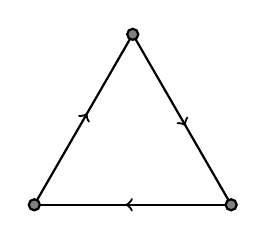
\begin{tikzpicture}[thick,scale=0.5]
			\draw[-<-] (0,0) to (5,0);
			\draw[-<-] (5,0) node{} to (60:5);
			\draw[-<-] (60:5) node{} to (0,0) node{};
		  \end{tikzpicture}
		& \ds{\{x_3^3-1, x_2-x_3z^2, x_1-x_3z\}}\\
	\hline
		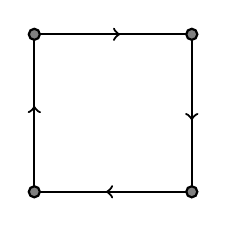
\begin{tikzpicture}[thick,scale=0.4]
		\draw[-<-] (0,0) -- (5,0);
		\draw[-<-] (5,0) node{} -- (5,5);
		\draw[-<-] (5,5) node{} -- (0,5);
		\draw[-<-] (0,5) node{} -- (0,0) node{};
		\end{tikzpicture}
		& \ds{\{x_4^4-1, x_3-x_4z^3, x_2-x_4z^2, x_1-x_4z\}}\\
	\hline
		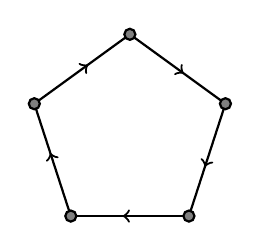
\begin{tikzpicture}[thick,scale=0.3]
		\draw[-<-] (0,0) -- (5,0);
		\draw[-<-] (5,0) node{} -- ++(72:5);
		\draw[-<-] (5,0)++(72:5) node{} -- ++(2*72:5);
		\draw[-<-] (5,0)++(72:5)++(2*72:5) node{} -- ++(3*72:5);
		\draw[-<-] (5,0)++(72:5)++(2*72:5)++(3*72:5) node{} -- (0,0) node{};
		\end{tikzpicture}
		& \ds{\{x_5^5-1, x_4-x_5z^4, x_3-x_5z^3, x_2-x_5z^2, x_1-x_5z\}}\\
	\hline
		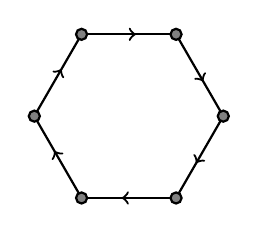
\begin{tikzpicture}[thick,scale=0.3]
		\draw[-<-] (0,0) -- (4,0);
		\draw[-<-] (4,0) node{} -- ++(60:4);
		\draw[-<-] (4,0)++(60:4) node{} -- ++(2*60:4);
		\draw[-<-] (4,0)++(60:4)++(2*60:4) node{} -- ++(3*60:4);
		\draw[-<-] (4,0)++(60:4)++(2*60:4)++(3*60:4) node{} -- ++(4*60:4);
		\draw[-<-] (4,0)++(60:4)++(2*60:4)++(3*60:4)++(4*60:4) node{} -- (0,0) node{};
		\end{tikzpicture}
		& \ds{\{x_6^6-1, x_5-x_6z^5, x_4-x_6z^4, x_3-x_6z^3, x_2-x_6z^2, x_1-x_6z\}}\\
	\hline
		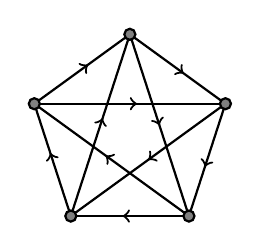
\begin{tikzpicture}[thick,scale=0.3]
		\draw[->-] (5,0)++(72:5) -- (0,0);
		\draw[-<-] (5,0)++(72:5)++(2*72:5) -- (0,0);
		\draw[->-] (5,0)++(72:5)++(2*72:5) -- (5,0);
		\draw[-<-] (108:5) -- (5,0);
		\draw[-<-] (5,0) ++(72:5) -- (108:5);
		\draw[-<-] (0,0) -- (5,0);
		\draw[-<-] (5,0) node{} -- ++(72:5);
		\draw[-<-] (5,0)++(72:5) node{} -- ++(2*72:5);
		\draw[-<-] (5,0)++(72:5)++(2*72:5) node{} -- ++(3*72:5);
		\draw[-<-] (5,0)++(72:5)++(2*72:5)++(3*72:5) node{} -- (0,0) node{};
		\end{tikzpicture}
		& {$\begin{aligned}\{& x_5^5-1, x_4^2+(z^3+z+1)x_4x_5+zx_5^2, x_3+(z^3+z+1)x_4+zx_5,\\& x_2+(z^2+1)x_4+(z^3+1)x_5, x_1+(-z^3-z^2-z-1)x_4+(-z^3-z)x_5\}\end{aligned}$}\\
	\hline
		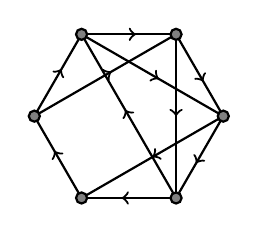
\begin{tikzpicture}[thick,scale=0.3]
		\draw[->-] (4,0)++(60:4) -- (0,0);
		\draw[-<-] (4,0)++(60:4)++(2*60:4)++(3*60:4) -- (4,0);
		\path (4,0)++(60:4)++(2*60:4)++(3*60:4) coordinate(farpoint);
		\draw[-<-] (4,0)++(60:4) -- (farpoint);
		\draw[->-] (4,0)++(60:4)++(2*60:4) -- (4,0);
		\draw[-<-] (4,0)++(60:4)++(2*60:4) -- (120:4);
		\draw[-<-] (0,0) -- (4,0);
		\draw[-<-] (4,0) node{} -- ++(60:4);
		\draw[-<-] (4,0)++(60:4) node{} -- ++(2*60:4);
		\draw[-<-] (4,0)++(60:4)++(2*60:4) node{} -- ++(3*60:4);
		\draw[-<-] (4,0)++(60:4)++(2*60:4)++(3*60:4) node{} -- ++(4*60:4);
		\draw[-<-] (4,0)++(60:4)++(2*60:4)++(3*60:4)++(4*60:4) node{} -- (0,0) node{};
		\end{tikzpicture}
		& {$\begin{aligned}\{& x_6^6-1, x_5+(z-1)x_6, x_4^2+x_4x_6+x_6^2, 3x_3+(z+1)x_4+(2z+2)x_6,\\& 3x_2+(2z-1)x_4+(-2z+1)x_6, x_1+(-z+1)x_4+(-z+1)x_6\}\end{aligned}$}\\
	\hline
		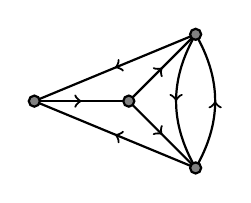
\begin{tikzpicture}[thick, scale=0.3]
		\path (4,0)++(45:4) coordinate(upper);
		\path (4,0)++(-45:4) coordinate(lower);
		\draw[->-] (upper) to (0,0);
		\draw[->-] (lower) to (0,0);
		\draw[->-] (upper) to[bend right] (lower);
		\draw[->-] (lower) to[bend right] (upper);
		\draw[->-] (0,0) node{} to (4,0);
		\draw[->-] (4,0) to ++(45:4) node{};
		\draw[->-] (4,0) node{} to ++(-45:4) node{};
		\end{tikzpicture}
		& \ds{\{x_4^4-1, x_3^2+x_4^2, 2x_2+(z+1)x_3+(z+1)x_4, 2x_1+(-z+1)x_3+(-z+1)x_4\}}\\
	\hline
		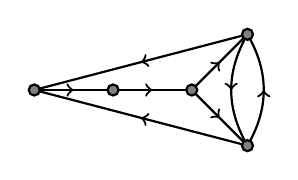
\begin{tikzpicture}[thick, scale=0.25]
		\path (4,0)++(45:4) coordinate(upper);
		\path (4,0)++(-45:4) coordinate(lower);
		\draw[->-] (upper) to (-4,0);
		\draw[->-] (lower) to (-4,0);
		\draw[->-] (upper) to[bend right] (lower);
		\draw[->-] (lower) to[bend right] (upper);
		\draw[->-] (-4,0) node{} to (0,0);
		\draw[->-] (0,0) node{} to (4,0);
		\draw[->-] (4,0) to ++(45:4) node{};
		\draw[->-] (4,0) node{} to ++(-45:4) node{};
		\end{tikzpicture}
		& {$\begin{aligned}\{& x_5^5-1, x_4^2+(z^3+z^2+1)x_4x_5+x_5^2, x_3+(z^2+1)x_4+(z^2+1)x_5,\\& x_2+(-z^3-z^2-1)x_4+(-z^3-z^2-1)x_5, x_1+(z^3+1)x_4+(z^3+1)x_5\}\end{aligned}$}\\
	\hline
		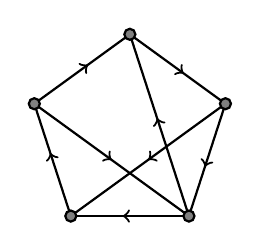
\begin{tikzpicture}[thick,scale=0.3]
		\draw[->-] (5,0)++(72:5) -- (0,0);
		\draw[-<-] (5,0)++(72:5)++(2*72:5) -- (5,0);
		\draw[->-] (108:5) -- (5,0);
		\draw[-<-] (0,0) -- (5,0);
		\draw[-<-] (5,0) node{} -- ++(72:5);
		\draw[-<-] (5,0)++(72:5) node{} -- ++(2*72:5);
		\draw[-<-] (5,0)++(72:5)++(2*72:5) node{} -- ++(3*72:5);
		\draw[-<-] (5,0)++(72:5)++(2*72:5)++(3*72:5) node{} -- (0,0) node{};
		\end{tikzpicture}
		& {$\begin{aligned}\{& x_5^5-1, x_4+(z^3+z^2+z+1)x_5, x_3^2+(-z^3-z)x_3x_5+(-z^3-z^2-z-1)x_5^2,\\& x_2+(z^3+z+1)x_3+x_5, x_1+(-z^3-z)x_3+(-z^3-z^2-z-1)x_5\}\end{aligned}$}\\
	\hline
		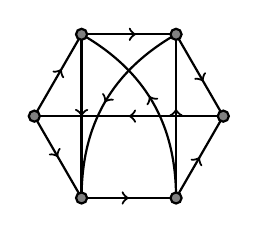
\begin{tikzpicture}[thick,scale=0.3]
		\path (4,0)++(60:4)++(2*60:4)++(3*60:4) coordinate(farpoint);
		\draw[->-] (4,0)++(60:4) -- (120:4);
		\draw[->-] (farpoint) -- (0,0);
		\draw[-<-] (4,0)++(60:4)++(2*60:4) -- (4,0);
		\draw[->-] (4,0)++(60:4)++(2*60:4) to[bend right] (0,0);
		\draw[-<-] (farpoint) to[bend left] (4,0);
		\draw[->-] (0,0) -- (4,0);
		\draw[->-] (4,0) node{} -- ++(60:4);
		\draw[-<-] (4,0)++(60:4) node{} -- ++(2*60:4);
		\draw[-<-] (4,0)++(60:4)++(2*60:4) node{} -- ++(3*60:4);
		\draw[-<-] (4,0)++(60:4)++(2*60:4)++(3*60:4) node{} -- ++(4*60:4);
		\draw[->-] (4,0)++(60:4)++(2*60:4)++(3*60:4)++(4*60:4) node{} -- (0,0) node{};
		\end{tikzpicture}
		& {$\begin{aligned}\{& x_6^6-1, x_5^3+2zx_5^2x_6+(2z-2)x_5x_6^2-x_6^3, x_4+x_5^2x_6^5+(z+1)x_5+(2z-1)x_6,\\& x_3+(z-1)x_5, x_2-x_5^2x_6^5+(-2z+1)x_5+(-z+2)x_6, x_1-zx_6\}\end{aligned}$}\\
	\hline
		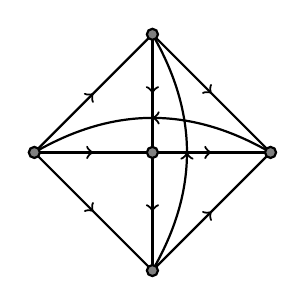
\begin{tikzpicture}[thick, scale=0.3]
		\draw[->-] (0,0) to (5,0);
		\draw[->-] (0,0) to (5,5);
		\draw[->-] (0,0) to (5,-5);
		\draw[->-] (5,5) to (5,0);
		\draw[->-] (5,0) to (5,-5);
		\draw[->-] (5,-5) to[bend right] (5,5);
		\draw[->-] (5,5) node{} to (10,0);
		\draw[->-] (5,0) node{} to (10,0);
		\draw[->-] (5,-5) node{} to (10,0);
		\draw[->-] (10,0) node{} to[bend right] (0,0) node{};
		\end{tikzpicture}
		& {$\begin{aligned}\{& x_5^5-1, x_4^3+(z+1)x_4^2x_5+(z^2+z+1)x_4x_5^2+(z^3+z^2+z+1)x_5^3,\\& 5x_3+(-z^3-2z^2-3z-4)x_4^2x_5^4+(2z^3-z^2+z+3)x_4\\&+(-z^3-2z^2+2z+1)x_5,\\& 5x_2+(z^3+2z^2+3z+4)x_4^2x_5^4+(-2z^3+z^2-z+2)x_4+(z^3+2z^2+3z+4)x_5,\\& x_1-zx_5\}\end{aligned}$}\\
	\hline
		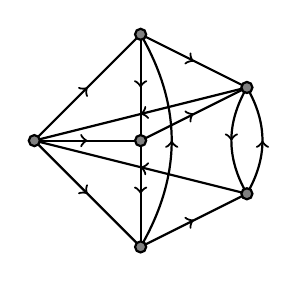
\begin{tikzpicture}[thick, scale=0.27]
		\draw[->-] (0,0) to (5,0);
		\draw[->-] (0,0) to (5,5);
		\draw[->-] (0,0) to (5,-5);
		\draw[->-] (5,5) to (5,0);
		\draw[->-] (5,0) to (5,-5);
		\draw[->-] (5,-5) to[bend right] (5,5);
		\draw[->-] (5,5) node{} to (10,2.5);
		\draw[->-] (5,0) node{} to (10,2.5);
		\draw[->-] (5,-5) node{} to (10,-2.5);
		\draw[->-] (10,2.5) to[bend right] (10,-2.5);
		\draw[->-] (10,-2.5) to[bend right] (10,2.5);
		\draw[->-] (10,2.5) node{} to (0,0);
		\draw[->-] (10,-2.5) node{} to (0,0) node{};
		\end{tikzpicture}
		& {$\begin{aligned}\{& x_6^6-1, x_5^2-x_5x_6+x_6^2, x_4x_5+(z-1)x_4x_6+(z-1)x_5x_6-zx_6^2,\\& x_4^2+(-z+2)x_4x_6+2x_5x_6+(z-1)x_6^2, x_3+(z+1)x_4+2zx_5,\\& 3x_2-3zx_4+(-4z+2)x_5+(2z+2)x_6, 3x_1+(-2z+1)x_5+(-2z+1)x_6\}\end{aligned}$}\\
	\hline
		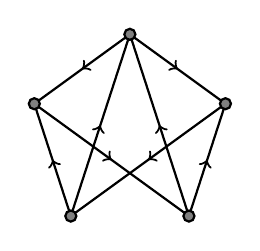
\begin{tikzpicture}[thick, scale=0.3]
		\path (5,0)++(72:5)++(2*72:5)++(3*72:5) coordinate(fifth);
		\path (5,0)++(72:5)++(2*72:5) coordinate(fourth);
		\path (5,0)++(72:5) coordinate(third);
		\draw[->-] (0,0) to (fifth);
		\draw[->-] (0,0) to (fourth);
		\draw[->-] (5,0) to (third);
		\draw[->-] (5,0) to (fourth);
		\draw[->-] (third) to (0,0) node{};
		\draw[->-] (fourth) to (third) node{};
		\draw[->-] (fourth) node{} to (fifth);
		\draw[->-] (fifth) node{} to (5,0) node{};
		\end{tikzpicture}
		& {$\begin{aligned}\{& x_5^5-1, x_4^2+(-z^3-z^2)x_4x_5+x_5^2, x_3+(z^3+z^2+z+1)x_4,\\& x_2+(z^3+z^2+z+1)x_5, x_1+(-z^3-z^2-z)x_4+(-z^3-z^2-z)x_5\}\end{aligned}$}\\
	\hline
		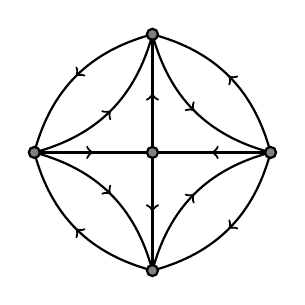
\begin{tikzpicture}[thick,scale=0.3]
		\draw[->-] (0,0) to (5,0);
		\draw[->-] (0,0) to[bend right] (5,5);
		\draw[->-] (0,0) to[bend left] (5,-5);
		\draw[->-] (5,0) to (5,5);
		\draw[->-] (5,0) to (5,-5);
		\draw[->-] (5,5) to[bend right] (0,0);
		\draw[->-] (5,5) to[bend right] (10,0);
		\draw[->-] (5,-5) to[bend left] (0,0) node{};
		\draw[->-] (5,-5) to[bend left] (10,0);
		\draw[->-] (10,0) to (5,0) node{};
		\draw[->-] (10,0) to[bend right] (5,5) node{};
		\draw[->-] (10,0) node{} to[bend left] (5,-5) node{};
		\end{tikzpicture}
		& {$\begin{aligned}\{& x_5^5-1, x_4^3+(z^3+1)x_4^2x_5+(z^3+z+1)x_4x_5^2-z^2x_5^3,\\& x_3x_4+(z^3+z^2+z+1)x_3x_5+(z+1)x_4^2+(z^2+z+1)x_5^2,\\& x_3^2+(-z^3-z)x_3x_5+(-z^3-z^2-z-1)x_5^2,\\& x_2+(-z^3-z)x_3+x_4, x_1+(z^3+z+1)x_3+x_5\}\end{aligned}$}\\
	\hline
\end{longtable}
\end{center}


%------------------------
% Hajos Construction
%------------------------

\section{Open Problems} \label{problems}

The study of Gr\"obner bases is relevant to many different fields, with many examples appearing in \cite{coxlittleoshea}. A specific conjecture which remains unproven after the course of writing this paper is as follows.
\begin{conjecture}
	Let $G$ be a graph with $n$ vertices, and $k \geq 2$. There exists $g$ in the reduced Gr\"obner basis of $H_G$ such that $\mathrm{LT}(g) = x_i^k$ for some $i$ such that $1 \leq i < n$ if and only if $G$ has more than one Hamiltonian cycle.
\end{conjecture}
Note that the forward direction is already known to be true from Theorem \ref{intersection}, so all that remains is to prove the other direction.

By carefully studying the requirements on the structure of $H_G$ from the graph polynomials, it may be possible to prove or disprove conjectures related to Hamiltonian cycles in graphs. A specific example is Sheehan's Conjecture.
\begin{conjecture}
	Every 4-regular graph has at least two Hamiltonian cycles.
\end{conjecture}
We hope that results and techniques studied in this paper can be used to study the issue of graph Hamiltonicity in more depth, and can also be applied to other algebraic problems.

\bibliographystyle{plain}
%\bibliography{references}



\begin{thebibliography}{9}

\bibitem{coxlittleoshea}
	Cox, Little, O'Shea,
	\emph{Ideals, Varieties, and Algorithms}.
	Springer, New York,
	Third Edition,
	2007.

\bibitem{deloera07}
	J.A. De Loera, J. Lee, S. Margulies, S. Onn,
	\emph{Expressing Combinatorial Optimization Problems by Systems of Polynomial Equations and the Nullstellensatz}.
	Unpublished.

\bibitem{deloera10}
	J.A De Loera, C. Hillar, P.N. Malkin, M. Omar,
	\emph{Recognizing Graph Theoretic Properties with Polynomial Ideals}.
	Unpublished.

\bibitem{hillar06}
	C. Hillar, T. Windfeldt,
	\emph{Algebraic Characterization of Uniquely Vertex Colorable Graphs}.
	Unpublished.

\end{thebibliography}


\end{document}
